% !TEX TS-program = pdflatex
% !TEX encoding = UTF-8 Unicode

\section{Projektmanagement}



\section{Das optische Tee-Tassen-Thermometer ($oT^3$)}

\subsection{Anforderungen}

\begin{table}[h]

\begin{center}
\tikzset{ 
    table/.style={
        matrix of nodes,
        row sep=-\pgflinewidth,
        column sep=-\pgflinewidth,
        nodes={
            rectangle,
            draw=black,
            align=center
        },
        minimum height=1.5em,
        text depth=0.5ex,
        text height=2ex,
        nodes in empty cells,
%%
        every even row/.style={
            nodes={fill=gray!20}
        },
        column 1/.style={
            nodes={text width=0.5\textwidth}
        },
        row 1/.style={
            nodes={
                fill=black!90,
                text=white,
                font=\bfseries
            }
        }
    }
}

\begin{tikzpicture}
\matrix (first) [table,text width=6em]
{
   Anforderungen   & leicht & mittel & schwer \\
   Schaltung           &       &        &   \\
   Programm          &       &        &   \\
   Aufbau                &       &       &    \\
};
 \end{tikzpicture}
\end{center}
\caption{}
\label{tab:}
\end{table}%



\section{Das eigene Motor Arduino Shield}

\subsection{Anforderungen}
\begin{table}[h]

\begin{center}

\tikzset{ 
    table/.style={
        matrix of nodes,
        row sep=-\pgflinewidth,
        column sep=-\pgflinewidth,
        nodes={
            rectangle,
            draw=black,
            align=center
        },
        minimum height=1.5em,
        text depth=0.5ex,
        text height=2ex,
        nodes in empty cells,
%%
        every even row/.style={
            nodes={fill=gray!20}
        },
        column 1/.style={
            nodes={text width=0.5\textwidth}
        },
        row 1/.style={
            nodes={
                fill=black!90,
                text=white,
                font=\bfseries
            }
        }
    }
}

\begin{tikzpicture}
\matrix (first) [table,text width=6em]
{
   Anforderungen   & leicht & mittel & schwer \\
   Schaltung           &       &        &   \\
   Programm          &       &        &   \\
   Aufbau                &       &       &    \\
};
 \end{tikzpicture}
\end{center}
\caption{}
\label{tab:}
\end{table}%

\subsection{Projektbeschreibung}

\section{SchulBot ein autonomes Fahrzeug}

\subsection{Anforderungen}
\begin{table}[h]
 \begin{center}
  \tikzset{ 
    table/.style={
        matrix of nodes,
        row sep=-\pgflinewidth,
        column sep=-\pgflinewidth,
        nodes={
            rectangle,
            draw=black,
            align=center
        },
        minimum height=1.5em,
        text depth=0.5ex,
        text height=2ex,
        nodes in empty cells,
%%
        every even row/.style={
            nodes={fill=gray!20}
        },
        column 1/.style={
            nodes={text width=0.5\textwidth}
        },
        row 1/.style={
            nodes={
                fill=black!90,
                text=white,
                font=\bfseries
            }
        }
    }
}

  \begin{tikzpicture}
\matrix (first) [table,text width=6em]
{
   Anforderungen   & leicht & mittel & schwer \\
   Schaltung           &       &        &   \\
   Programm          &       &        &   \\
   Aufbau                &       &       &    \\
};
 \end{tikzpicture}
\end{center}
\caption{}
\label{tab:}
\end{table}%

\subsection{Projektbeschreibung}
Teilautonom oder autonom gesteuerte Fahrzeug spielen eine immer größer werdende Rolle in unsere modernen Gesellschaft. In moderne Autos steuern Mikrocontroller Fahrerassistenzsysteme wie z.B. ABS. Diese Technik wird zur Zeit weiterentwickelt. Im Mai 2012 erhielt Google die erste Zulassung eines autonomen Fahrzeugs in den USA. So erlaubte der US-Bundesstaat Nevada den Test des selbstfahrenden Autos auf öffentlichen Straßen. Bedingung ist jedoch, dass sich eine Person hinter dem Steuer befindet, die notfalls eingreifen kann.
\marginfigure{Kapitel4/Bilder/Google_driverless_car}{Google autonomous car}{fig:google_driverless_car}

Im Bereich der Transportfahrzeuge gibt es schon seit längerem automatisierte fahrerlose Fahrzeuge. Fahrerlose Transportsysteme (FTS) sind innerbetriebliche, flurgebundene Fördersysteme mit automatisch gesteuerten Fahrzeugen, deren primäre Aufgabe der Materialtransport, nicht aber der Personentransport ist. Sie werden innerhalb und außerhalb von Gebäuden eingesetzt und bestehen im Wesentlichen aus folgenden Komponenten: 
\begin{itemize}
\item einem oder mehreren Fahrerlosen Transportfahrzeugen
\item einer Leitsteuerung
\item Einrichtungen zur Standortbestimmung und Lageerfassung
\item Einrichtungen zur Datenübertragung
\item Infrastruktur und peripheren Einrichtungen.
\end{itemize}
\marginfigure{Kapitel4/Bilder/Unterfahrschlepper-FTF}{Fahrerlose Transportsystem als Unterfahrschlepper}{fig:ftf}


\subsection{Aufgabenstellung}

Ihr sollte ein autonomes Roboterfahrzeug planen, bauen und programmieren. 
Das Fahrzeug soll folgende Aufgaben lösen.  

\subsubsection{Aufgabe 1}
Das Fahrzeug soll mindestens 10 Meter gerade aus fahren und dabei maximal 1 Meter nach links 
oder rechts abweichen.

\subsubsection{Aufgabe 2}
Euer Fahrzeug soll mit Hilfe zweier Schalter Wände erkennen und dieses Ausweichen. 

\subsubsection{Aufgabe 3}
Euer Fahrzeug soll mit Hilfe eines Optokopplers eine schwarze Linie erkennen und dieser folgen. 


\subsection{Material}

Vorgefertigter Bauplan, zwei Getriebemotoren, Arduino Uno mit ProjektShield, Batteriehalter, 
Grundplatte  

\subsubsection{Fertigungstechniken}
CNC Fräsen, Löte, 


\subsection{Erstellung des Bauplans}

Mit Hilfe der CAD/CAM Software nccad plant und entwerft ihr auf Grundlage der Vorlage 
mcgbot.cad die Bodenplatte eures Fahrzeuges. 

\begin{figure}[htbp]
\begin{center}
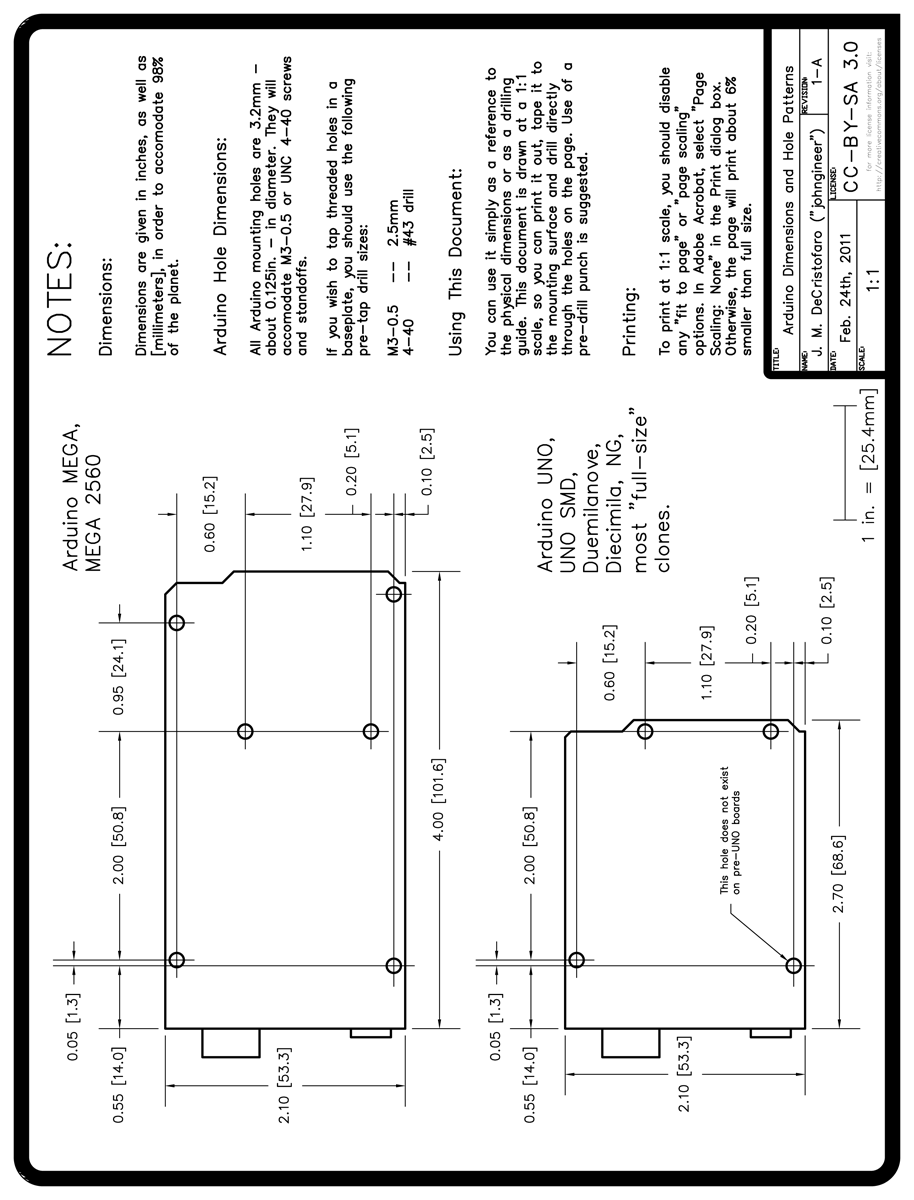
\includegraphics[width=0.7\textwidth,angle=-90]{Kapitel4/Bilder/arduino_dimension}
\caption{default}
\label{default}
\end{center}
\end{figure}


\section{Paperduino-UNO, das selbstgebaute Arduino-Board}

\subsection{Anforderungnen}

\begin{table}[h]

\begin{center}
\tikzset{ 
    table/.style={
        matrix of nodes,
        row sep=-\pgflinewidth,
        column sep=-\pgflinewidth,
        nodes={
            rectangle,
            draw=black,
            align=center
        },
        minimum height=1.5em,
        text depth=0.5ex,
        text height=2ex,
        nodes in empty cells,
%%
        every even row/.style={
            nodes={fill=gray!20}
        },
        column 1/.style={
            nodes={text width=0.5\textwidth}
        },
        row 1/.style={
            nodes={
                fill=black!90,
                text=white,
                font=\bfseries
            }
        }
    }
}

\begin{tikzpicture}
\matrix (first) [table,text width=6em]
{
   Anforderungen   & leicht & mittel & schwer \\
   Schaltung           &       &        &   \\
   Programm          &       &        &   \\
   Aufbau                &       &       &    \\
};
 \end{tikzpicture}
\end{center}
\caption{}
\label{tab:}
\end{table}%

\subsection{Projektbeschreibung}

\begin{figure}[htbp]
\begin{center}
\subfigure[Schaltplan]{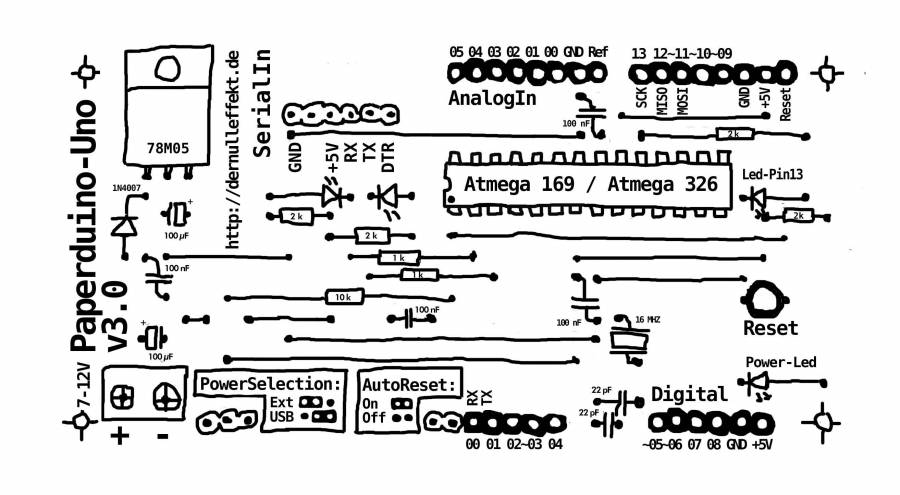
\includegraphics[width=0.4\textwidth]{Kapitel4/Bilder/Paperduino-Uno_30}}
\subfigure[Fertige Platine]{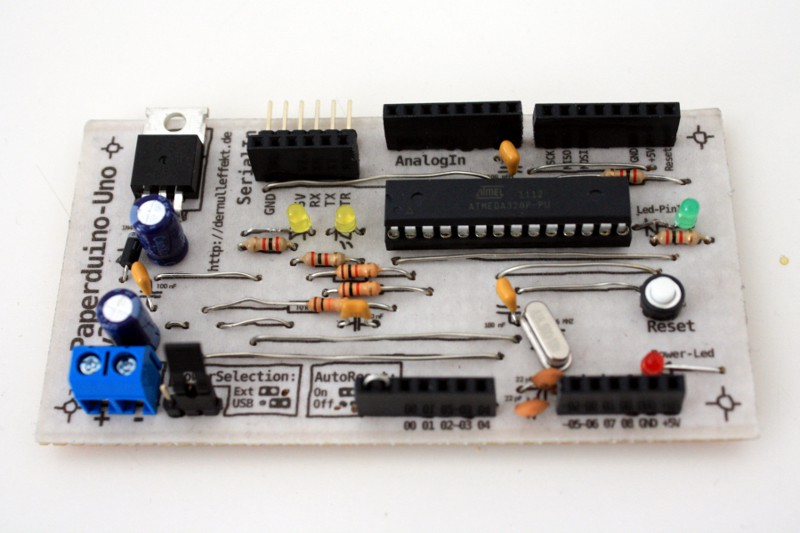
\includegraphics[width=0.4\textwidth]{Kapitel4/Bilder/paperduino-uno-30}}
\caption{default}
\label{default}
\end{center}
\end{figure}


\section{Roboter Arm}

\subsection{Anforderungnen}

\begin{table}[h]

\begin{center}
\tikzset{ 
    table/.style={
        matrix of nodes,
        row sep=-\pgflinewidth,
        column sep=-\pgflinewidth,
        nodes={
            rectangle,
            draw=black,
            align=center
        },
        minimum height=1.5em,
        text depth=0.5ex,
        text height=2ex,
        nodes in empty cells,
%%
        every even row/.style={
            nodes={fill=gray!20}
        },
        column 1/.style={
            nodes={text width=0.5\textwidth}
        },
        row 1/.style={
            nodes={
                fill=black!90,
                text=white,
                font=\bfseries
            }
        }
    }
}

\begin{tikzpicture}
\matrix (first) [table,text width=6em]
{
   Anforderungen   & leicht & mittel & schwer \\
   Schaltung           &       &        &   \\
   Programm          &       &        &   \\
   Aufbau                &       &       &    \\
};
 \end{tikzpicture}
\end{center}
\caption{}
\label{tab:}
\end{table}%

\subsection{Projektbeschreibung}